\subsection{Multi-Task Imitation Learning}
\label{sec:occp_mtil}
The methods discussed in the Section \ref{sec:lfd} describe architectures and approaches specifically designed to solve a single task, with limited generalization to the object category (e.g., picking blocks rather than balls) and initial state (e.g., the object starting position). For instance, a system trained for pick-and-place operations cannot be repurposed for tasks like assembly operations. The methods described here address these limitations, solving the problem of \textit{Multi-Task Imitation Learning} (MTIL).

Before starting to present and describe the different methods and approaches, it is necessary to describe the problem. Starting from a reformulation of the dataset used to train the system and the learned policy.
Indeed, in Section~\ref{sec:problem_formulation}, the expert dataset $\mathcal{D}^{E}$ has been introduced. Based on the problem to solve this dataset can composed in different way. Specifically, in the context of MTIL, the dataset $\mathcal{D}^{E}$ can be seen as a composition of $n$ datasets, $\mathcal{D}^{E}=\left \{\mathcal{D}_{1}, \dots, \mathcal{D}_{n}\right \}$, where $\mathcal{D}_{i} = \left \{ (\tau_{m_{i}}^{j}, \ c_{m_{i}}), j=1,\dots,N, \ m_{i} \in \mathcal{M}_{i}\right \}$ is the \textit{single-task dataset}, composed of:
\begin{itemize}
    \item $N$ expert demonstration for each $m^{th}$ variation of the $i^{th}$ task, where $M_{i}$ is the number of variation for the $i^{th}$ task.
    \item Agent trajectories $\tau_{m_{i}}^{j} = (s_{0}, a_{0}, s_{1}, a_{1}, \dots, a_{T-1}, s_{T})$. where $s_{t}$ is the state at time $t$ and $a_{t}$ is the corresponding action (Section \ref{sec:problem_formulation}).
    \item Task-conditioning signal $c_{m_{i}}$ for the $m^{th}$ variation of $i^{th}$ task, which describes the desired task in terms of video demonstrations \cite{james2018task_embedded,bhutani2022attentive_one_shot,dasari2021transformers_one_shot,mandi2022towards_more_generalizable_one_shot}, natural language description \cite{stepputtis2020language,jang2022bc_z,mees2022calvin,doasIcan2022,mees2022hulc,brohan2022rt,shridhar2023perceiver} or multi-modal prompt, that exploits both visual information (e.g., an image of the target object) and text information that contains the information related to the action to be performed \cite{jiang2023vima}.
\end{itemize}
The goal of Multi-Task Imitation Learning is to learn a \textit{conditioned policy} $\pi^{L}_{\theta}(a_{t}|s_{t}, c_{m_{i}})$, that is able to map the current state and command into the corresponding action.
Depending on how the policy is defined, various loss functions come into play. In the case of deterministic policies, the learning process focuses on minimizing the Mean-Squared Error (refer to Formula \ref{eq:mse}). However, for probabilistic policies, the learning process centers around minimizing the Negative Log-likelihood (refer to Formula \ref{eq:nll}). This approach aims to enhance the probability of correctly executing the action.
% \begin{equation}
%     \label{eq:mse}
%     \mathcal{L}(D^{E}, \pi^{L}_{\theta}) = \frac{1}{n} \sum_{\mathcal{D}^{i} \sim \mathcal{D}^{E}} \frac{1}{N} \sum_{(\tau_{m_{i}}^{j}, c_{m_{i}}) \sim \mathcal{D}^{i}} \frac{1}{T}\sum_{t=0}^{T} (a_{t} - \pi^{L}_{\theta}(s_{t}, c_{m_{i}}))
% \end{equation}
% \begin{equation}
%     \label{eq:nll}
%     \mathcal{L}(D^{E}, \pi^{L}_{\theta}) = \frac{1}{n} \sum_{\mathcal{D}^{i} \sim \mathcal{D}^{E}} \frac{1}{N} \sum_{(\tau_{m_{i}}^{j}, c_{m_{i}}) \sim \mathcal{D}^{i}} \frac{1}{T}\sum_{t=0}^{T} (a_{t} - \pi^{L}_{\theta}(s_{t}, c_{m_{i}}))
% \end{equation}

\begin{equation}
    \label{eq:mse}
    \mathcal{L}(\tau_{m_{i}}^{j}, c_{m_{i}},\pi^{L}_{\theta}) = \frac{1}{T}\sum_{t=0}^{T} (a_{t} - \pi^{L}_{\theta}(s_{t}, c_{m_{i}}))^{2}
\end{equation}
\begin{equation}
    \label{eq:nll}
    \mathcal{L}(\tau_{m_{i}}^{j}, c_{m_{i}},\pi^{L}_{\theta}) = - \frac{1}{T}\sum_{t=0}^{T} log(\pi^{L}_{\theta}(a_{t}|s_{t}, c_{m_{i}}))
\end{equation}
The following sections will describe the various approaches proposed to address the problem. Figure \ref{fig:mtil_taxonomy} illustrates the taxonomy used for the Multi-Task Imitation Learning methods. Specifically, the methods are categorized based on the type of generalization required by the algorithm (Few-Shot vs. Zero-Shot). For Few-Shot generalization, the Meta-Learning paradigm will be discussed, as it is most relevant to the problem at hand. For Zero-Shot generalization, the methods are further divided based on the type of conditioning signal used, whether it is provided through natural language descriptions or visual information.
\begin{figure}[t]
    \centering
    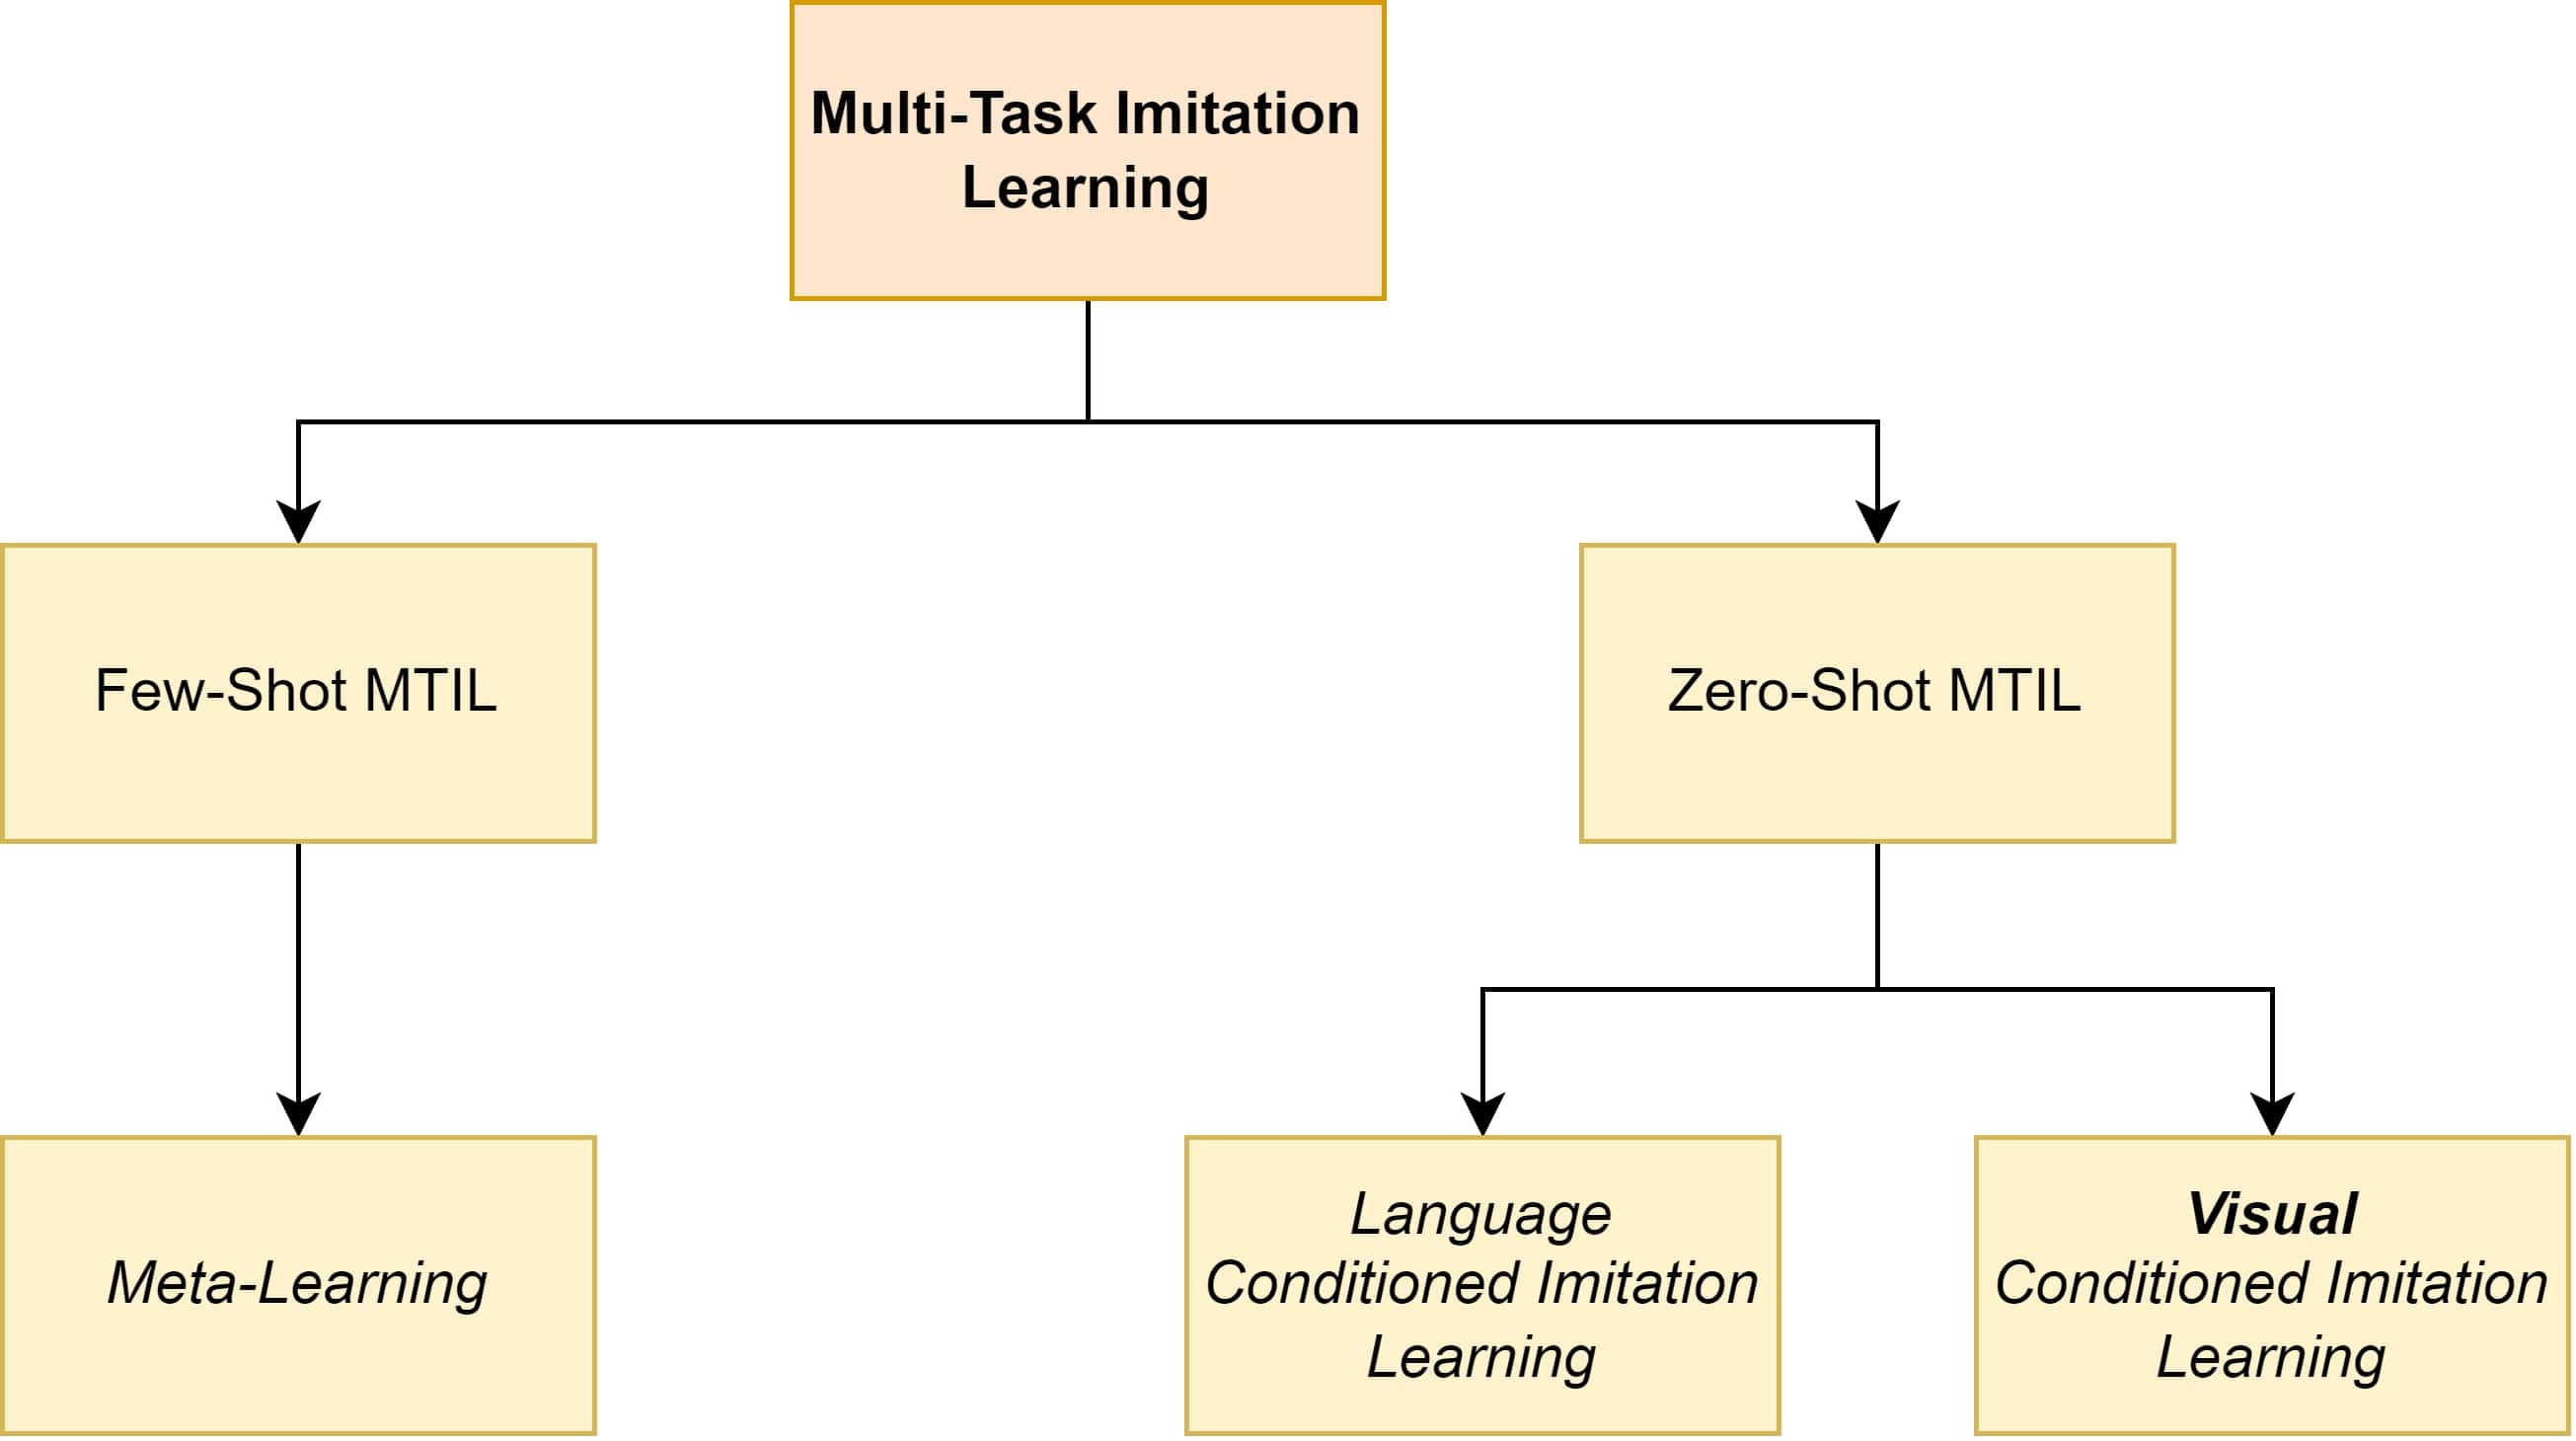
\includegraphics[width=0.8\textwidth]{figures/images/MTIL_taxonomy.jpg}
    \caption{Multi-Task Imitation Learning Taxonomy.}
    \label{fig:mtil_taxonomy}
    
\end{figure}


\textbf{Few-Shot MTIL} refers to approaches designed to train a model on a variety of tasks so that it can effectively solve a new task using only few samples and consequently requires only a few back-propagation steps \cite{finn2017maml}. In this context, one of the most significant learning paradigms, especially relevant to robotic manipulation, is \textit{Meta-Learning}. The goal of Meta-Learning is to train a model that can ``learn to learn," meaning it develops a set of general weights $\theta$ that, while not directly usable for solving any specific task within a distribution of tasks $\mathcal{T}$, can be quickly adapted through a few backpropagation steps to solve a given task within that distribution, $\mathcal{T}_{i} \in \mathcal{T}$. One of the most popular Meta-Learning algorithms is the \textit{Model-Agnostic Meta-Learning} (MAML) algorithm \cite{finn2017maml}, described in Algorithm \ref{alg:maml}. The MAML algorithm follows an iterative learning procedure consisting of two steps:
\begin{itemize}
    \item \textbf{Meta-Learning}: During this phase, task-specific weights $\theta_{i}$ are computed for each sampled task $\mathcal{T}_{i}$. Specifically, the \textit{meta-parameters} $\theta$ are updated according to the gradient obtained from evaluating the loss function on the $i^{th}$ task $\mathcal{T}_{i}$, where the function $f$ is parameterized by the meta-parameters $\theta$.

    \item \textbf{Meta-Adaptation}: In this phase, the meta-parameters are further refined. The loss function $f$, now parameterized by the task-specific parameters for the $i^{th}$ task, is used to adjust the meta-parameters based on the gradients derived from the sum of the loss functions evaluated on the task-specific weights. This process provides feedback to the meta-parameters $\theta$ from each task, leading to a generalized point that can be easily adapted to new tasks (Figure \ref{fig:maml_weights}).
\end{itemize}
\begin{algorithm}[t]
\caption{Model-Agnostic Meta-Learning (MAML) \cite{finn2017maml}}
\label{alg:maml}
\begin{algorithmic}
\REQUIRE Distribution over tasks $p(\mathcal{T})$
\STATE Randomly initialize $\theta$
\WHILE {$i=1, \dots N$}
    \STATE Sample batch of tasks $ \mathcal{T}_{i} \sim p(\mathcal{T})$
    \FOR {\textbf{all} $\mathcal{T}_{i}$}
        \STATE Evaluate $\nabla_\theta \mathcal{L}_{\mathcal{T}_{i}}(f_{\theta})$ w.r.t. $K$ examples
        \STATE Compute adapted parameters with gradient descent: $\theta'_{i} = \theta - \alpha \nabla_\theta\mathcal{L}_{\mathcal{T}_{i}}(f_{\theta})$
    \ENDFOR
    \STATE Update $\theta \leftarrow \theta - \beta \nabla_\theta \sum_{\mathcal{T}_{i} \sim p(\mathcal{T})} \mathcal{L}_{\mathcal{T}_{i}}(f_{\theta'_{i}})$
\ENDWHILE
\end{algorithmic}
\end{algorithm}
\begin{figure}[tb]
    \centering
    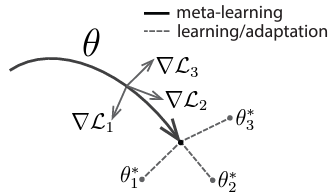
\includegraphics[width=0.6\textwidth]{figures/images/maml_weights.png}
    \caption{Diagram of MAML algorithm, which optimizes for a representation $\theta$ that can quickly adapt to new tasks}
    \label{fig:maml_weights}
\end{figure}

The MAML algorithm is the base for different methods which apply Few-Shot Imitation Learning in the context of Behavioral Cloning \cite{finn2017one_shot_visual_il,yu2018daml,yu2018one_shot_hil}.

In \cite{finn2017one_shot_visual_il}, MAML algorithm was used to prove the effectiveness of Meta-Learning in the context of real robot manipulation, with visual observations, as opposite to \cite{duan2017one_shot_il}. A Convolutional Neural Network was trained by following the Algorithm \ref{alg:maml}, using as loss-function the Mean Squared Error, computed between the predicted action and the ground truth one. For real-robot experiments a dataset of \textbf{1300} placing demonstrations (i.e., place an holded object in a target container), containing near to \textbf{100} different objects, was collected through teleportation. The trained system was tested by performing the adaptation step on one video demonstration, over 29 new objects, moreover, between the video demonstration and the actual execution, the objects configuration was changed. In this setting the system reached the $\mathbf{90\%}$ of success rate, outperforming baseline methods based on LSTM \cite{duan2017one_shot_il}, and contextual network (i.e., a Convolutional Neural Network that takes in input the current observation and the image representing the target state).

In \cite{yu2018daml}, the \textit{Domain Adaptive Meta-Learning} algorithm (DAML) was proposed with the goal of learning to infer a policy from a single human demonstration. To achieve it, a two-step algorithm was proposed. In the first-step, called \textbf{Meta-Learning step}, given in input, for each task $\mathcal{T}$, a set of human demo $\mathcal{D}^{h}_{\mathcal{T}}$ and a set or robot demo $\mathcal{D}^{r}_{\mathcal{T}}$ (Figure \ref{fig:daml_tasks}), the \textit{initial policy parameters} $\theta$ and the \textit{adaptive loss} parameters $\psi$ are learned, solving the problem in Formula \ref{eq:daml}.
\begin{equation}
 \label{eq:daml}
 \underset{\theta,\psi}{\min} \sum_{\mathcal{T} \sim p(\mathcal{T})} \sum_{\mathbf{d}^{h} \sim D^{h}_{\mathcal{T}}} \sum_{\mathbf{d}{^r} \sim D^{r}_{\mathcal{T}}} \mathcal{L}_{BC}(\theta - \alpha \nabla_\theta\mathcal{L}_{\psi}(\theta,\mathbf{d}^{h}), \mathbf{d}^{r})
\end{equation}

\newline The outer loss is the classic supervised Behavioral Cloning loss, defined as $\mathcal{L}_{BC}(\phi, \mathbf{d^{r}}) = \sum_{t} \log(\pi_{\phi}(a_{t} \mid s_{t}, o_{t}))$. The inner loss, $\mathcal{L}_{\psi}$, is a learned \textbf{adaptive loss}. Specifically, $\mathcal{L}_{\psi}$ is used during Meta-Adaptation, where the policy parameters are updated by evaluating the gradients derived from $\mathcal{L}_{\psi}$. This process involves using a video of a human demonstrating a new task $\mathcal{T}$ as input, leading to the policy update defined by $\phi_{\mathcal{T}} = \theta - \alpha \nabla_{\theta} \mathcal{L}_{\psi}(\theta, \mathbf{d}^{h})$. 
\newline This adaptive loss is the key component proposed in DAML. To use it effectively, it is necessary to learn the parameters $\psi$, observing how there is no direct correspondence between the human video demonstration and the robot's ground truth actions. To address this challenge, the authors of DAML observed that while the policy learns to produce appropriate actions through the $\mathcal{L}_{BC}$ loss, the adaptive loss should instead adjust the perceptual aspect of the policy, focusing on human motion and the manipulated object. Based on this insight, the authors implemented the function $\mathcal{L}_{\psi}$ using a 1D Temporal Convolutional Network (Figure \ref{fig:daml_temporal_adaptation_loss}). The convolutional layers are applied to a stack of embeddings generated by the policy $\pi$ across different frames of the video demonstrations. The parameters of this module are learned during the meta-training phase, following the weight update process described in Formula \ref{eq:daml_temporal_adaptation_loss}. The objective of $\mathcal{L}_{\psi}$ is to generate task-specific policy parameters $\phi_{\mathcal{T}}$ that guide the policy to produce effective actions.

\begin{equation}
 \label{eq:daml_temporal_adaptation_loss}
 \begin{matrix}
    (\theta, \psi) \leftarrow(\theta, \psi)-\beta \nabla_{\theta, \psi} \mathcal{L}_{\mathrm{BC}}\left(\phi_{\mathcal{T}}, \mathbf{d}^r\right) \\ \\
   \phi_{\mathcal{T}}=\theta-\alpha \nabla_\theta \mathcal{L}_\psi\left(\theta, \mathbf{d}^h\right)
   \end{matrix}
\end{equation}

\newline Experimental evaluation on tasks such as placing, pushing, and pick-and-place, has shown that: \begin{itemize}
    \item The system was able to generalize across both new objects and objects configuration starting from only a single human demonstration;
    \item A performance degradation was observed in large domain-shift experiments, such as novel backgrounds and different camera view-points.
\end{itemize}
\begin{figure}[t]
    \centering
    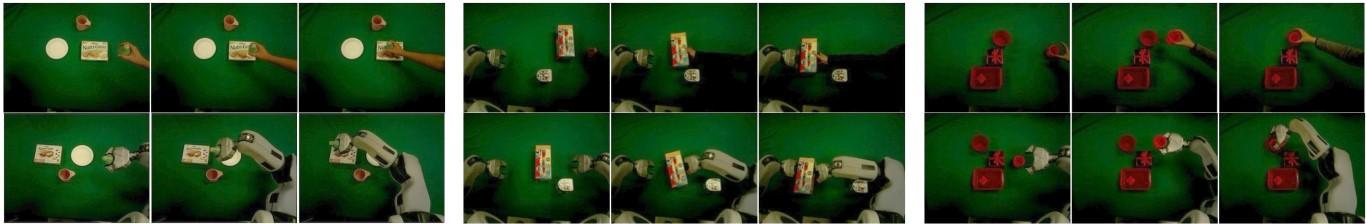
\includegraphics[width=\textwidth]{figures/images/daml/tasks.jpg}
    \caption{Tasks performed in \cite{yu2018daml}. (Top row) Human demonstration, (Bottom row) robot demonstration. (Left) Placing task, (Middle) pushing task, (Right) pick-and-place task.}
    \label{fig:daml_tasks}
\end{figure}

\begin{figure}[t]
    \centering
    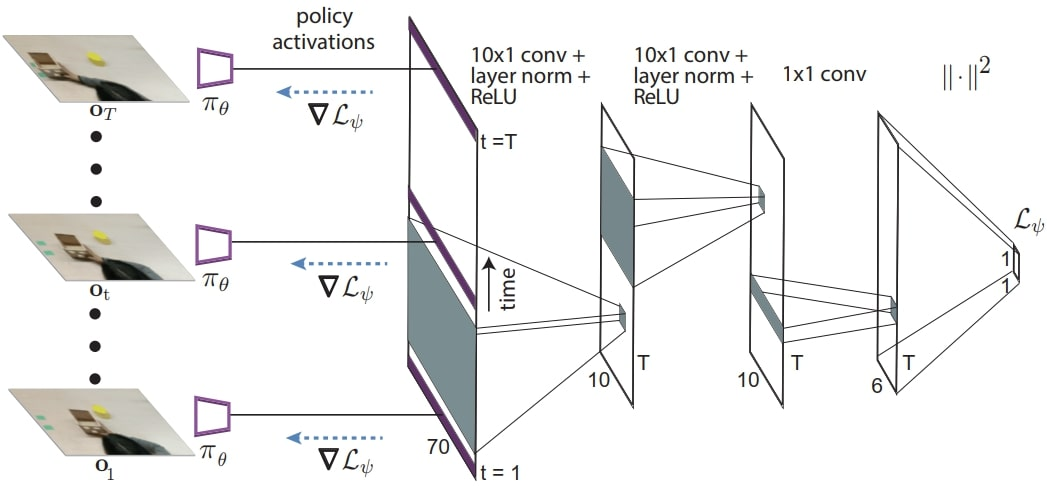
\includegraphics[width=0.8\textwidth]{figures/images/daml/daml_temporal_adaptation_loss.jpg}
    \caption{The Temporal Adaptation Loss architecture applies 1D temporal convolutional layers to the stacked embeddings generated by the policy $\pi$ from the frames of the human video demonstration.}
    \label{fig:daml_temporal_adaptation_loss}
\end{figure}

Meta-Learning algorithms have demonstrated interesting properties, notably their capacity for few-shot generalization to novel objects and object configurations. However, it has been observed that during the adaptation step, these methods tend to lose their effectiveness in performing other tasks. This limitation has underscored the need for the development of Multi-Task Imitation Learning methods, which aim to address these shortcomings and enable more versatile task execution in complex scenarios. These kinds of methods will be discussed in the following paragraphs.

\textbf{Zero-Shot MTIL} refers to approaches that aim to train a model capable of solving different tasks without any further adaptation or backpropagation steps. This approach addresses a key issue in Meta-Learning methods, which is the problem of forgetting how to solve previous tasks after adapting to a new one. The goal is to develop a single policy that can handle multiple tasks in a zero-shot manner.

In this context, a crucial design choice is how to convey the desired task to the policy. The literature identifies two main methods to address this problem:

\begin{enumerate}
    \item \textit{Language Conditioned}: These methods leverage natural language descriptions of tasks to inform the model about the task to be executed.
    \item \textit{Visual Conditioned}: These methods use visual information (e.g., goal-state images, video demonstrations) to provide the model with the task instructions.
\end{enumerate}

\textit{Language Conditioned}, as said a possible and intuitive way to inform the policy about which task to execute is through natural language description. Indeed, by looking to the phrase ``Pick the blue cube and place it in the red bow'', there are both information about the action to perform (pick and place) and which are the objects involved (blue cube and red bow). Consequently, through training a neural network with a diverse set of tasks, the system should exhibit the ability to generalize its understanding to both previously unseen objects within familiar tasks and entirely novel tasks composed of the fundamental actions practiced during training. This approach showcases the potential for \textbf{robust} and \textbf{adaptable} \textbf{human-robot interaction} in real-world scenarios.

Foundational research, such as that by \cite{stepputtis2020language} and \cite{jang2022bc_z}, has sought to explore the previously mentioned hypothesis. Notably, \cite{stepputtis2020language} introduced an innovative architectural framework, depicted in Figure \ref{fig:language_conditioned}, marking the first instance of seamlessly integrating language, vision, and control tasks. This model is composed of two critical components: a \textit{Semantic Model}, which generates a task embedding denoted as $e$ by processing the initial scene image and the accompanying text command, and a \textit{Control Model}, which generates the control signal using the current robot state $r_{t}$ and the task embedding $e$.

A crucial aspect of such architectures is the management of the visual state, represented by the image $I$, and the command $v$, to create a meaningful embedding $e$ that encapsulates both the current scene state and the desired command. Specifically, the image is first processed using a pre-trained object detection network (Faster R-CNN \cite{fastrcnn}) to identify salient objects in the robot's environment. The detected objects are represented by feature vectors, which include class and bounding box information. Concurrently, the language command is embedded into a suitable representation using a language embedding technique (e.g., GloVe \cite{pennington2014glove}), with the command vector $V$ encoded by a recurrent GRU unit. To associate the objects identified with the sentence embedding $s$, a likelihood value is computed for each object proposal $a_{i} = w_{a}^{T} f_{a}([\text{f}_{i}, s])$, and a probability distribution is computed over the candidates $\mathbf{a} = \text{softmax}([a_0, \dots, a_c])$. Finally, the task embedding $e$ is formed by a fully connected layer that takes as input the sentence embedding $s$ and the weighted sum of object candidate features $e'= \sum_{i=0}^{c} f_{i}a_{i}$.

Training of this model was conducted on two fundamental tasks, namely ``Picking" and ``Pouring", within scenarios featuring multiple objects of the same category, which served as distractors (see Figure \ref{fig:objects}). The subsequent testing experiments demonstrated the system's capability to successfully complete the picking task 98 out of 100 times and the pouring task 85 out of 100 times within novel scenarios. These results serve as compelling evidence of the efficacy and potential of language-conditioned methodologies in the field.
\begin{figure}[t]
    \centering
    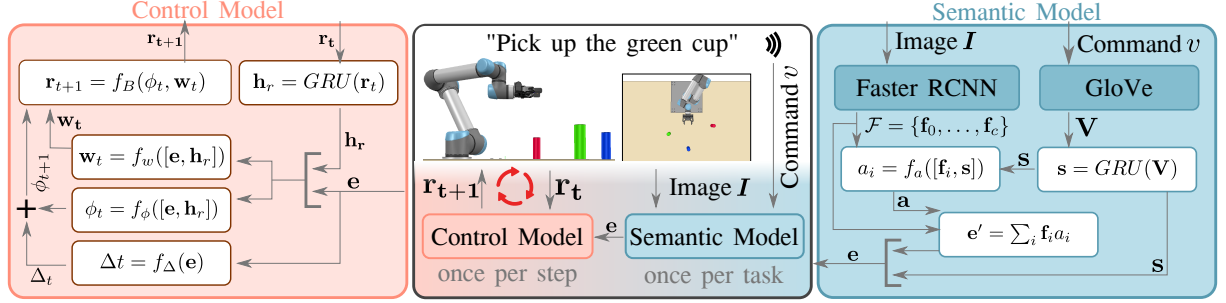
\includegraphics[width=0.9\textwidth]{figures/images/language_conditioned/architecture.png}
    \caption{Architecture proposed in \cite{stepputtis2020language}. The \textit{Semantic Model} takes in input the image $I$ and the command $v$, generating a command conditioned embedding $e$. The \textit{Control Module} receives in input the embedding $e$ and the current robot state $r_{t}$ and produces the next control signal.}
    \label{fig:language_conditioned}
\end{figure}

\begin{figure}[t]
    \centering
    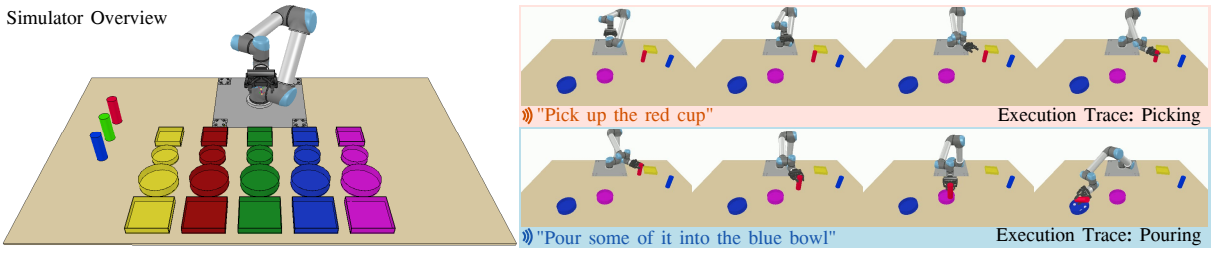
\includegraphics[width=0.9\textwidth]{figures/images/language_conditioned/objects.png}
    \caption{(Left) Set of object used in \cite{stepputtis2020language}. (Right) Sample of task execution (right)}
    \label{fig:objects}
\end{figure}


Authors in \cite{jang2022bc_z} make a step towards a more general agent, by proposing a large-scale dataset containing \textbf{100} diverse manipulation tasks. The demonstrations were collected through both expert teleoperation and shared autonomy process (HG-DAgger \cite{kelly2019hg_dagger}). The demonstrated tasks were related to pick-and-place, grasp, pick-and-drag, pick-and-wipe, and push skills. The dataset was used to train the network in Figure \ref{fig:bcz_architecture}. As it can be noted the samples were composed by the current robot observation, and a conditioning represented by either a \textit{\textbf{natural language description}} or a \textit{\textbf{human video demonstration}}.
The idea was that training a conditioned policy over the current observation $o_{t}$, and a task representation $c$, , it would allow the policy to generalize over new tasks in a zero-shot manner (i.e., without any fine-tuning). 
Specifically, in contrast to the previous method, this approach does not rely on pre-trained object detectors to identify candidate regions. Instead, the Task Embedding is directly injected into the Feature Maps generated by the Convolutional Neural Network ResNet-18. This injection is carried out through the FiLM layer \cite{perez2018film}.

Experimental results shown that, over 28 held-out tasks, containing both completely new objects, and known objects but in different tasks, an average success rate of \textbf{38\%} was reached in the easiest setting, with only one distractor and with natural language instruction. The success rate dropped to \textbf{4\%} in the hardest setting with 4 distractors and video conditioning.
\begin{figure}[t]
    \centering
    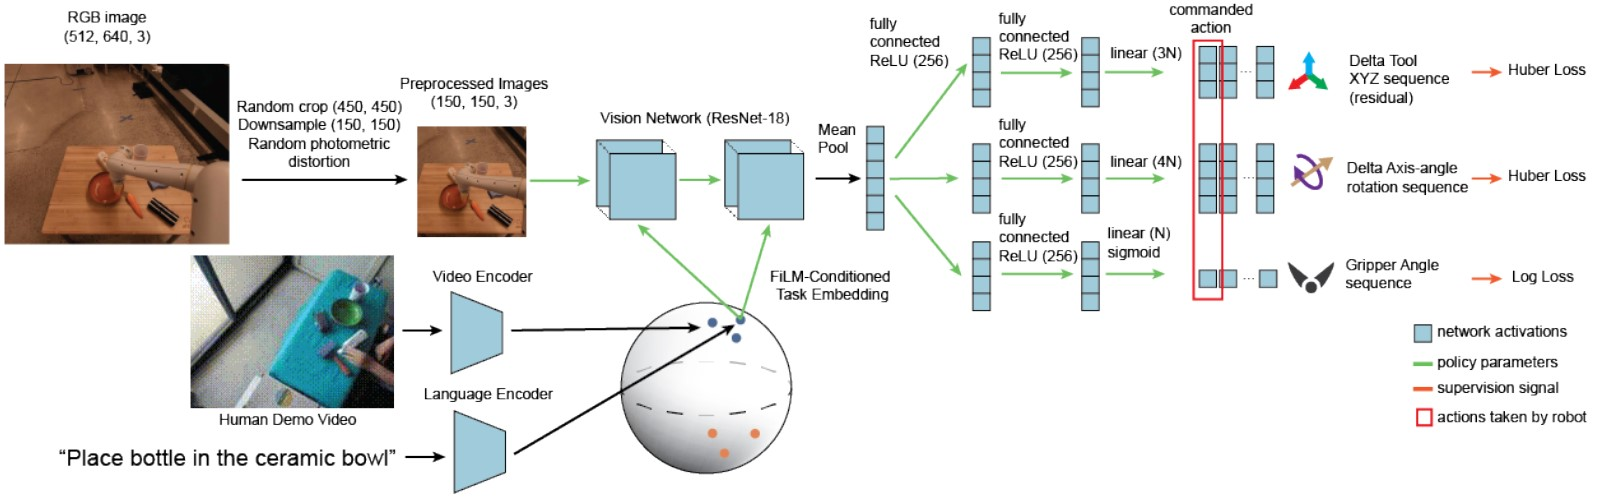
\includegraphics[width=0.9\textwidth]{figures/images/bc_z/bc-z-network.jpg}
    \caption{Architecture proposed in \cite{jang2022bc_z}. Here, the Task Embedding is injected directly in the Feature Maps generated by the ResNet-18.}
    \label{fig:bcz_architecture}
\end{figure}


Foundational research in the field of Language-Conditioned Multi-Task Imitation Learning has demonstrated promising results in zero-shot generalization. However, the robustness of their performance remains a challenge. Subsequent research, as highlighted in \cite{brohan2022rt,mees2022calvin,mees2022hulc}, has focused on enhancing performance. 

In particular, the authors of \cite{brohan2022rt} sought to investigate whether the transfer of knowledge from extensive, diverse, and task-agnostic datasets, which has enabled modern machine learning models to excel in zero or few-shot learning scenarios for new and specific tasks, is applicable within the realm of robotics. This inquiry arises due to the presence of high-capacity architectures capable of assimilating knowledge from such large datasets. To explore this prospect, the authors in \cite{brohan2022rt} introduced a comprehensive dataset comprising over 130,000 demonstrations collected across more than 700 household tasks (Figure \ref{fig:rt_1_dataset}). Additionally, they proposed a Language-Conditioned Transformer-based architecture (Figure \ref{fig:rt_1_model}). Here the authors made relevant modification in the architecture, with respect to the previous BC-Z architecture \cite{jang2022bc_z}.Indeed, they modified the Visual Module by using an EfficientNet \cite{tan2019efficientnet} instead of the ResNet-18. The instruction was encoded using the Universal Sentence Encoder \cite{cer2018universal}, and the policy was implemented through a Transformer. Additionally, the authors addressed the real-time constraints of robot control. To accelerate inference time and achieve a frequency of $3$ Hz, the authors employed a TokenLearner module \cite{ryoo2021tokenlearner}, which utilizes an attention mechanism to select the most relevant tokens, thereby reducing the number of tokens that the underlying control module must process to infer the action.
\begin{figure}[t]
    \centering
    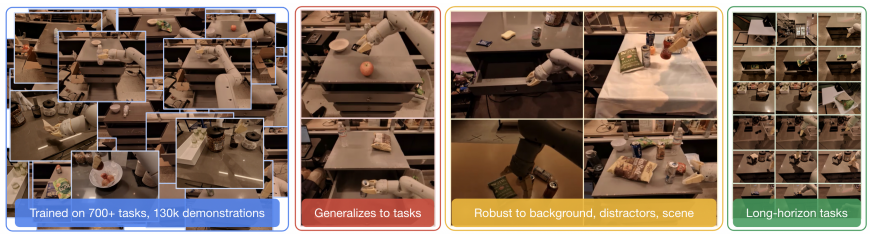
\includegraphics[width=0.8\textwidth]{figures/images/rt_1/dataset_image.png}
    \caption{Examples of household scenarios in RT-1 large-scale dataset.}
    \label{fig:rt_1_dataset}
\end{figure}

\begin{figure}[t]
    \centering
    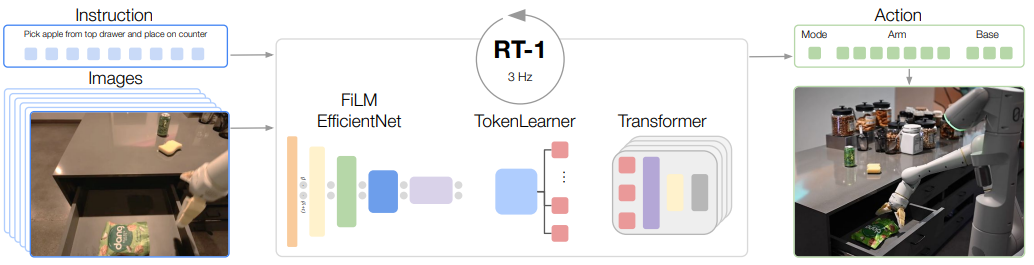
\includegraphics[width=\textwidth]{figures/images/rt_1/model.png}
    \caption{RT-1 Language-Conditioned Transformer based architecture proposed in \cite{brohan2022rt}.}
    \label{fig:rt_1_model}
\end{figure}
% \usepackage{graphicx}
% \usepackage{hhline}


\begin{table}
    \centering
    \caption{Distribution of tasks in large-scale dataset proposed in \cite{brohan2022rt}}
    \label{table:rf1_dataset}
    \resizebox{\linewidth}{!}{%
    \begin{tabular}{|c|c|c|c|} 
    \hline
    \textbf{Skill} & \textbf{Count} & \textbf{Description} & \textbf{Example Instruction} \\ 
    \hhline{|====|}
    Pick Object & 130 & Lift the object off the surface & pick iced tea can \\ 
    \hline
    Move Object Near Object & 337 & Move the first object near the second & move pepsi can near rxbar blueberry \\ 
    \hline
    Place Object Upright & 8 & Place an elongated object upright & place water bottle upright~ ~ \\ 
    \hline
    Knock Object Over & 8 & Knock an elongated object over & knock redbull can over \\ 
    \hline
    Open Drawer & 3 & Open any of the cabinet drawers & open the top drawer \\ 
    \hline
    Close Drawer & 3 & Close any of the cabinet drawers & close the middle drawer \\ 
    \hline
    Place Object into Receptacle & 84 & Place an object into a receptacle & place brown chip bag into white bowl \\ 
    \hline
    \begin{tabular}[c]{@{}c@{}}Pick Object from Receptacle\\and Place on the Counter\end{tabular} & 162 & \begin{tabular}[c]{@{}c@{}}Pick an object up from a location \\and then place it on the counter\end{tabular} & \begin{tabular}[c]{@{}c@{}}pick green jalapeno chip bag from\\~paper~bowl and place on counter\end{tabular} \\ 
    \hline
     & 9 & Skills trained for realistic, long instructions & \begin{tabular}[c]{@{}c@{}}open the large glass jar of pistachios \\~pull napkin out of dispenser grab scooper\end{tabular} \\ 
    \hhline{|====|}
    \textbf{Total} & 744 &  &  \\
    \hline
    \end{tabular}
    }
    \end{table}
It is worth noting the intriguing findings presented in Table \ref{table:rt1_results}. The model exhibits robustness in replicating tasks it has encountered before, and it even performs reasonably well on tasks it hasn't seen previously. However, a notable decline in performance becomes apparent when the model is exposed to novel backgrounds and scenarios featuring distracting objects, especially when the available data for these situations is limited. This observed trend holds significance because, unlike domains such as Computer Vision and Natural Language Processing where gathering large-scale datasets is relatively straightforward, the collection of real-world robotic datasets is a laborious and time-consuming endeavor. Furthermore, these real-world robotic datasets often have limited applicability to other research due to \textbf{disparities in action space, robot morphology, and scene representation}, as pointed out by \cite{brohan2022rt}. Therefore, the aspiration is to develop a system capable of replicating tasks with minimal demonstrations specifically gathered from the particular robot in use.
\newline Furthermore, the decline in success performance when faced with distractor objects emphasizes that addressing the policy-learning problem in an end-to-end manner, which involves mapping high-dimensional and high-level inputs like images and text directly to low-dimensional, low-level outputs such as the actions to be executed, may not be the most effective approach. This is because such models might lack the necessary perceptual components that enable them to initially recognize the target object within the scene, subsequently navigate towards it, and commence the manipulation process. This process aligns with how humans approach manipulation tasks \cite{grill2003neural}.
% \usepackage{graphicx}
% \usepackage{hhline}


\begin{table}
    \centering
    \caption{Results reported in \cite{brohan2022rt} by training the same model RT-1 with different dataset size.}
    \label{table:rt1_results}
    \resizebox{\linewidth}{!}{%
    \begin{tabular}{|c|c|c|c|c|c|c|c|} 
    \cline{5-8}
    \multicolumn{1}{c}{} & \multicolumn{1}{c}{} & \multicolumn{1}{c}{} &  & \multicolumn{4}{c|}{Generalization} \\ 
    \hline
    Models & \% Tasks & \% Data & Seen Tasks & All & Unseen Tasks & Distractors & Backgrounds \\ 
    \hhline{|========|}
    RT-1 & 100 & \textbf{100} & 97 & 73 & 76 & \textbf{83} & 59 \\ 
    \hline
    RT-1 & 100 & \textbf{51} & 71 & 50 & 52 & \textbf{39} & 59 \\ 
    \hline
    RT-1 & 100 & \textbf{37} & 55 & 46 & 57 & \textbf{35} & 47 \\ 
    \hline
    RT-1 & 100 & \textbf{22} & 59 & 29 & 14 & \textbf{31} & 41 \\
    \hline
    \end{tabular}
    }
    \end{table}

As we have seen up to now, all the proposed methods were tested on different robotic platforms with different scenarios and environments. As in other Computer Vision problem, there are no well now benchmark that are used by the researchers around the world. To solve this problem, authors in \cite{mees2022calvin} proposed CALVIN (Composing Actions from Language and Vision), which is an open-source simulated benchmark designed for learning long-horizon language-conditioned tasks in robotic manipulation. Specifically, CALVIN proposes a set of 34 manipulation tasks in 4 different environments (Figure \ref{fig:calvin_env}). 
\begin{figure}[t]
    \centering
    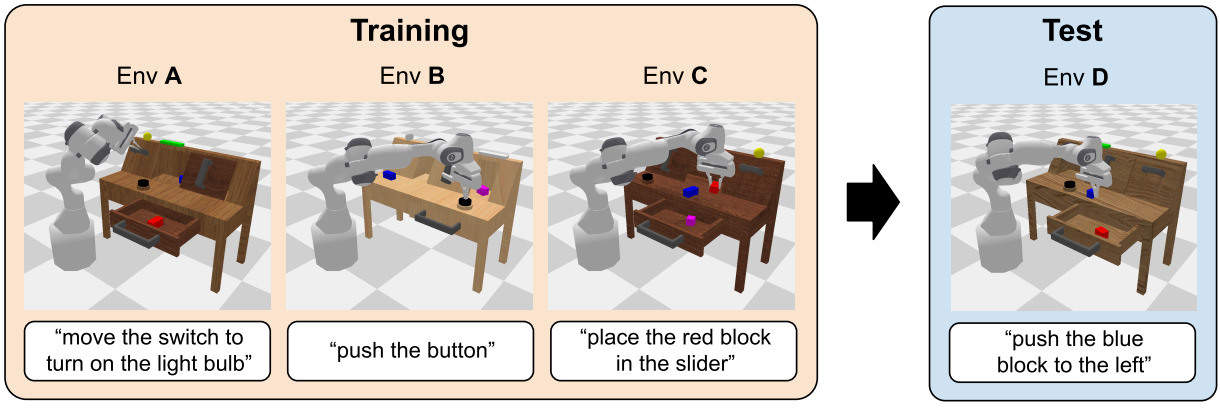
\includegraphics[width=0.9\textwidth]{figures/images/calvin/calvin_env.jpg}
    \caption{Environment proposed in CALVIN benchmark \cite{calvin}. The environments have different textures and all static elements such as the sliding door, the drawer, the light button, and switch are positioned differently}
    \label{fig:calvin_env}
\end{figure}
This benchmark was used by \cite{mees2022hulc,mees2023hulc++,reuss2024multimodal}. Specifically, the work proposed in \cite{reuss2024multimodal} is actually the best performing method on the CALVIN benchmark. The authors proposed an architecture that is able to handle goals described in terms of both natural language description and goal image, moreover they used a Diffusion Transformer Model as policy (Figure \ref{fig:mdt_architecture}). To reach this goal, the authors had to solve first the problem related to how to force the Multimodal Transformer Encoder to generate the same behavior independently of the goal modality. To solve this problem authors of MDT proposed two auxiliary self-supervised loss functions:
\begin{itemize}
    \item \textit{Masked Generative Foresight} (MGF) is a reconstruction-loss function designed to ensure that the MDT generates embeddings capable of guiding the robot behavior consistently across different modalities. This means that the tokens generated by the MDT can be used to construct image patches representing feature states, whether the goal is specified in terms of an image or a language description. Specifically, given the latent embedding of the MDT encoder for state $s_i$ and goal $g$, MGF trains a Vision Transformer (ViT) to reconstruct a sequence of 2D image patches $(u_1, \dots, u_U) = \text{patch}(s_{i+v})$ corresponding to the future state $s_{i+v}$.
    \item \textit{Contrastive Latent Alignment} (CLA) is a contrastive loss term designed to encourage the MDT to align the embeddings generated from a goal image with those generated from a language description. For each training sample $(s_i, a_i)$ paired with a multimodal goal specification $G_{s_i,a_i} = \{o_i, l_i\}$, CLA reduces the image and language goals to vectors $z_i^o$ and $z_i^l$, respectively. The CLA loss is then computed using the InfoNCE loss, based on the cosine similarity $C(z_i^o, z_i^l)$ between the image-goal conditioned state embedding $z_i^o$ and the language-goal conditioned state embedding $z_i^l$.
\end{itemize}
\begin{figure}[t]
    \centering
    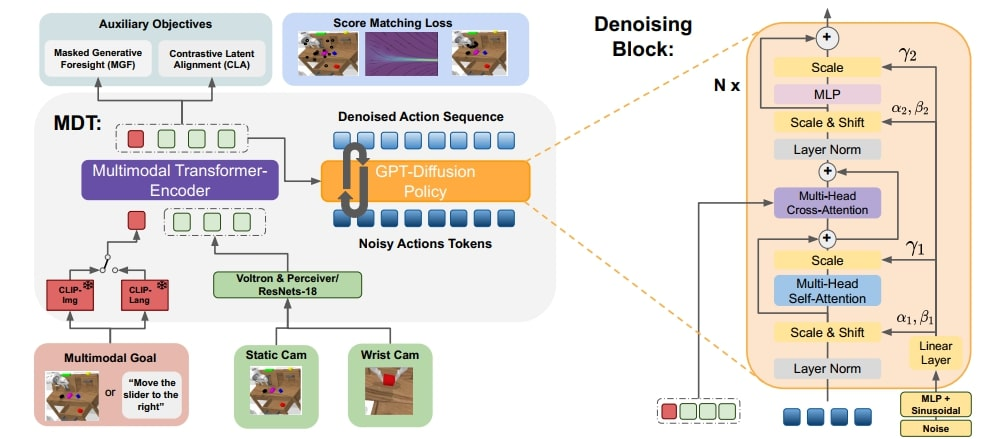
\includegraphics[width=\textwidth]{figures/images/mdt/mdt_architecture.jpg}
    \caption{The Multimodal Diffusion Transformer (MDT) architecture proposed in \cite{reuss2024multimodal}}
    \label{fig:mdt_architecture}
\end{figure}
As mentioned, this method was tested on the CALVIN benchmark, specifically in the $ABCD \rightarrow D$ test scenario, where the model was trained on the $ABCD$ environments and tested on environment $D$. The CALVIN benchmark comprises a set of 1000 rollouts, with each rollout consisting of a sequence of 5 commands. It is noteworthy that the MDT architecture successfully completed $80\%$ of the rollouts up to the fifth command. In particular, the MGF loss was observed to have a significant impact on system performance, improving the success rate for the fifth command from $69.8\%$ to $79.4\%$. This demonstrates that making the embedding informative about the system's evolution can meaningfully guide the diffusion system, which predicts actions over a certain time horizon into the future.

In the context of Language Conditioned MTIL, other important works to cite include \cite{shridhar2022cliport, shridhar2023perceiver}. Specifically, the authors in \cite{shridhar2022cliport} introduced CLIP-Port, a two-stream architecture that explicitly models the two key tasks in language-conditioned imitation learning: reasoning about \textbf{what to do} and reasoning about \textbf{how to do it}. The former task, referred to as \textit{semantic reasoning}, is derived from the text-based command and is handled using a pre-trained CLIP architecture \cite{radford2021learning}. The latter task, known as \textit{spatial reasoning}, is managed by leveraging the Transporter architecture \cite{zeng2021transporter}. The overall architecture (Figure \ref{fig:clip_port_architecture}) is an Encoder-Decoder framework that ultimately outputs an \textbf{affordance map}, which identifies the locations for executing pick or place operations (Figure \ref{fig:clip_port_affordance}).

During testing, this method was not directly compared with other Language Conditioned MTIL approaches. However, the results obtained allow for several observations. Notably, for tabletop manipulation tasks, the ability to reason using both spatial and semantic features enables a high success rate (ranging from $80\%$ to $90\%$) on tasks involving seen object attributes, such as color, even with a relatively low number of demonstrations (100). However, similar to the results reported in Table \ref{table:rt1_results}, CLIP-Port also struggles with entirely novel tasks, as evidenced by a significant drop in performance when dealing with unseen object attributes and a lower number of demonstrations.

\begin{figure}[t]
    \centering
    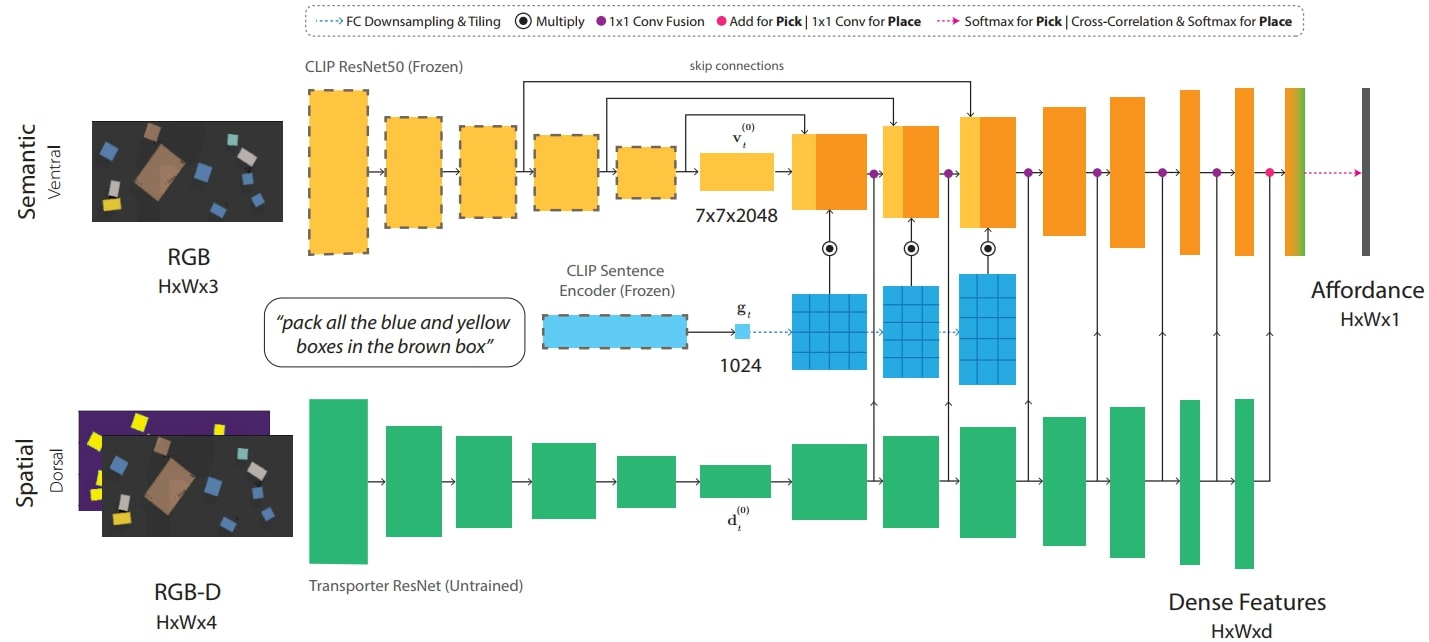
\includegraphics[width=\textwidth]{figures/images/clip_port/architecture.jpg}
    \caption{The Dual Stream architecture proposed in \cite{shridhar2022cliport} consists of two parallel streams: a semantic stream and a spatial stream. The semantic stream utilizes a frozen CLIP ResNet50 to encode the RGB input, with the decoder layers conditioned by tiled language features from the CLIP sentence encoder. Meanwhile, the spatial stream encodes the RGB-D input, and its decoder layers are laterally fused with those of the semantic stream. The final output is a map of dense pixelwise features, which is used to predict pick or place affordances.}
    \label{fig:clip_port_architecture}
\end{figure}

\begin{figure}[t]
    \centering
    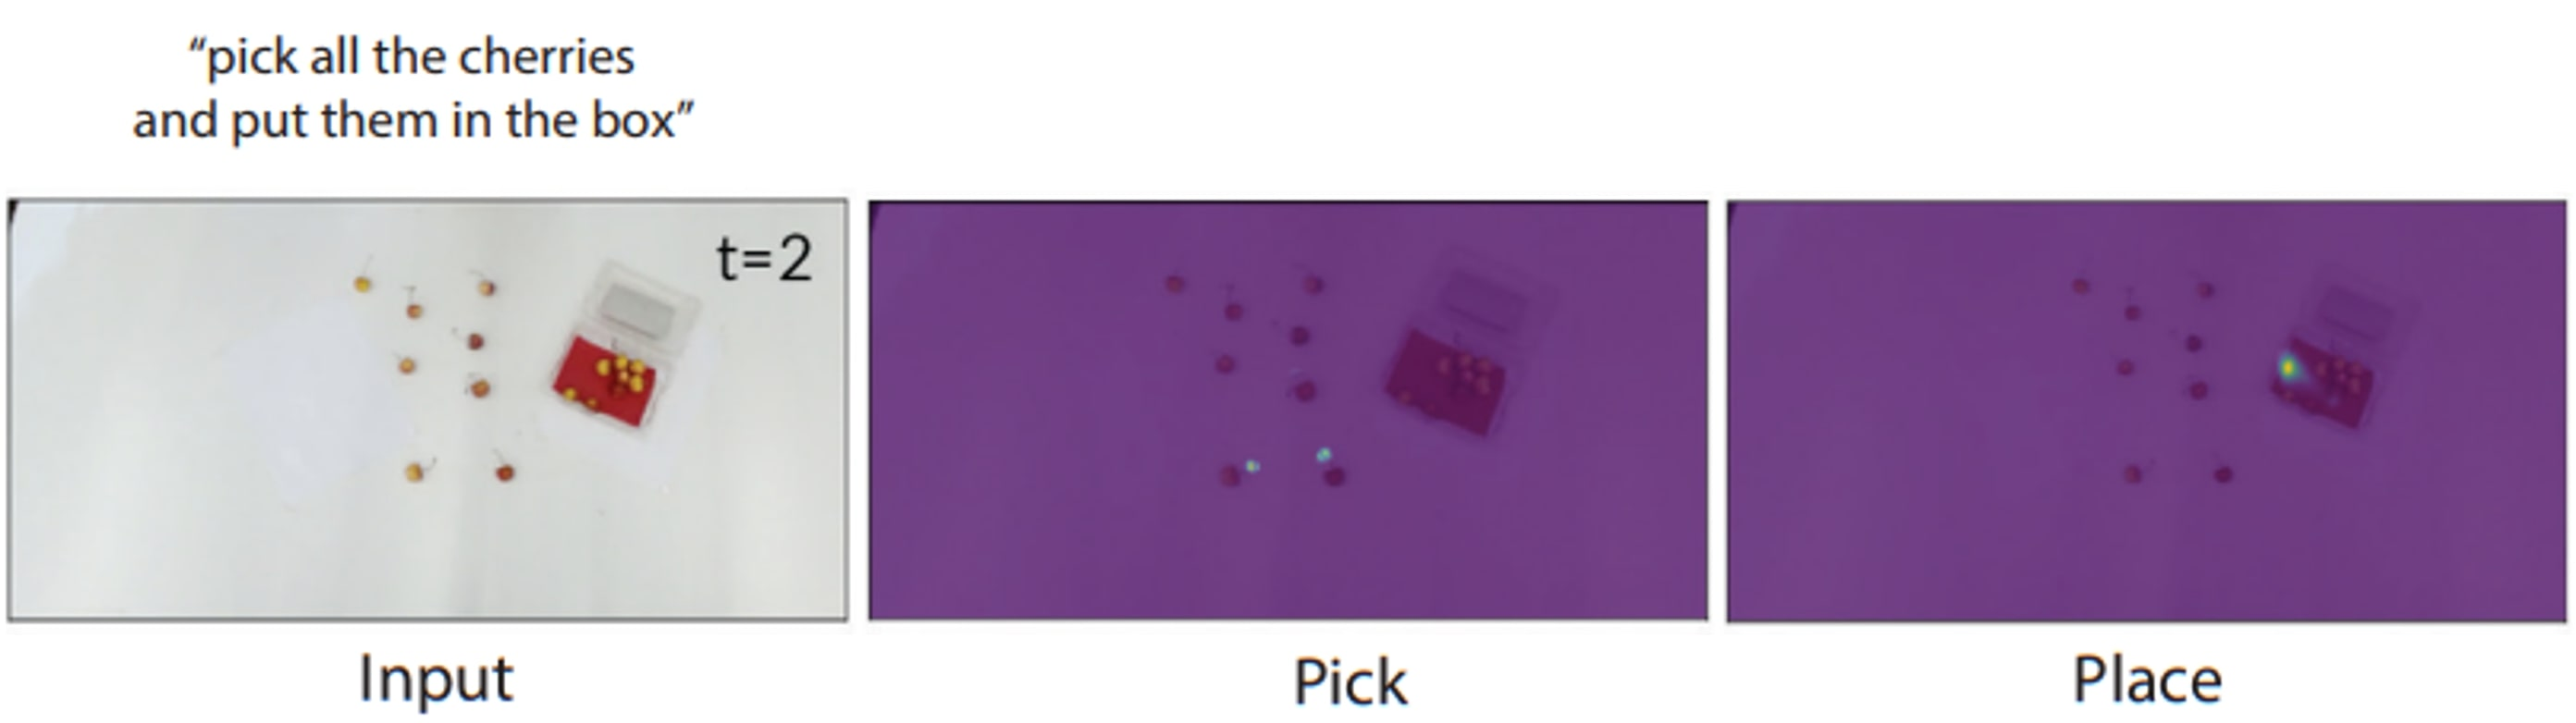
\includegraphics[width=0.8\textwidth]{figures/images/clip_port/affordance_map.jpg}
    \caption{Example of affordance map. (Left) The top-view input image. (Center) The affordance map for the pick-operation, since the task is to grab cherries the map highlights the two pickable cherries. (Right) The affordance map for the place operation.}
    \label{fig:clip_port_affordance}
\end{figure}

In conclusion, as discussed in this paragraph, considerable research effort has been dedicated to addressing the problem of Language Conditioned MTIL, particularly in terms of architectural designs and learning strategies. However, it remains challenging to draw definitive conclusions from these various approaches, as they are generally not evaluated on a common benchmark. Despite this issue, some trends can be observed. There is clearly room for improvement in the generalization capabilities of these methods, particularly in handling novel scenarios and tasks. Additionally, data efficiency remains a concern, as there is a noticeable decline in performance as the number of expert trajectories decreases. Another challenge is the ability to manage cluttered scenes with \textbf{relevant distractors}, objects that may have been manipulated during training but must be ignored in the target task, which can lead to occlusion and/or confusion.

\textit{Visual Conditioned} refers to methods that use visual information as a conditional signal. This information can be represented either as an image depicting the desired goal state or as a sequence of frames illustrating how the task should be performed. The idea behind this kind of methods is to build systems that are able to replicate tasks by observing the execution performed by other agents, like human can learn task by mimicking the execution of other humans.

Preliminary works, such as those by \cite{james2018task_embedded} and \cite{bhutani2022attentive_one_shot}, introduced architectures conditioned on the first and last frames of task demonstrations. Specifically, in \cite{james2018task_embedded}, the authors proposed TecNets (Task-Embedded Control Networks), an architecture illustrated in Figure \ref{fig:task_embedded}. TecNets consist of two main components:

\begin{itemize}
    \item \textit{Task-Embedding Network}: The purpose of this network is to create an embedding space where demonstrations of the same task are closely clustered, while embeddings of different tasks are kept as distant as possible. This network is trained using a contrastive loss function, defined in Formula \ref{eq:task_loss}, which ensures that the embedding of the $k^{th}$ sample of the $j^{th}$ task is similar to the "sentence" representing that task (i.e., the average of the embeddings of the $j^{th}$ task) and maximizes the distance from the sentences of other tasks.
    \begin{equation}
        \label{eq:task_loss}
        \mathcal{L}_{emb} = \sum_{\tau^{j}_{k} \in \mathcal{T}^{j}}\sum_{ \mathcal{T}^{i} \notin \mathcal{T}^{j}} \max \left[ 0, \text{margin} - s^{j}_{k}\cdot s^j + s^{j}_{k}\cdot s^i \right]
    \end{equation}
    \item \textit{Control Network}: This module implements the policy $\pi$, which takes as input the current observation $o$ and the sentence $s$ of the desired task. It then generates the corresponding action for the robot, conditioned on the task.
\end{itemize}

\begin{figure}[t]
    \centering
    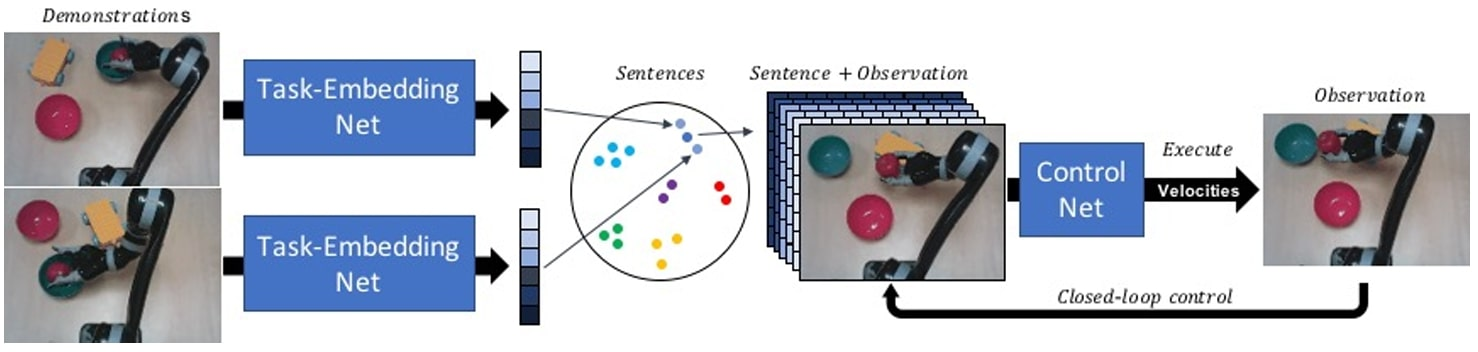
\includegraphics[width=\textwidth]{figures/images/task_embedded/task_embedded.jpg}
    \caption{Architecture proposed in \cite{james2018task_embedded}. The \textit{Task Embedding Net} generates the embedding representing the task to be performed given the goal image. The \textit{Control Net} implements the policy, and takes in input the current observation and the tiled task embedding.}
    \label{fig:task_embedded}
\end{figure}


The results from this preliminary work demonstrated the feasibility of training a vision-conditioned system capable of solving tasks in a zero-shot manner. The system achieved a success rate of \textbf{86.31}\% on a simulated 2D reaching task and \textbf{77.25}\% on a simulated pushing task. However, it is important to note a significant limitation of these approaches: the conditioning signal often fails to adequately capture critical information about the optimal strategy for solving the task. This shortcoming arises because the conditioning signal does not fully encode the strategies needed for effective task execution.


The methodologies introduced in \cite{dasari2021transformers_one_shot} and \cite{mandi2022towards_more_generalizable_one_shot} aim to advance the concept of an ideal multi-task agent, capable of replicating new tasks based on a single demonstration, often performed by another agent (e.g., a robot or a human).

In \cite{dasari2021transformers_one_shot}, the authors focused on training a vision-based control architecture (depicted in Figure \ref{fig:tosil_architecture}) that can replicate a task demonstrated through a set of frames sampled from a video of another agent performing the task. The architecture relies on two main components:
\begin{itemize}
    \item \textit{ResNet-18} \cite{resnet}, which serves as the backbone for extracting visual embeddings from the current agent state and the demonstration frames.
    \item \textit{Transformer} \cite{vaswani2017attention}, which uses the attention mechanism to combine embeddings from the demonstration frames with the current visual observation.
\end{itemize}

This architecture was trained using multiple loss terms, specifically:
\begin{itemize}
    \item \textit{Behavioral Cloning} term $\mathcal{L}_{BC}$ (Formula \ref{eq:tosil_bc}), a supervised loss function used to learn the action to perform given the agent's observation and the demonstrated task. Specifically, the loss function is a negative log-likelihood, computed over a mixture of learned logistic distributions, where the $i^th$ component is parameterized according to the mean and variance $(\mu_{i}, \sigma_{i})$ which are estimated through a MLPs.
    \begin{equation}
        \label{eq:tosil_bc}
        \mathcal{L}_{BC} = - ln(\sum_{i=0}^{k}\alpha_{i}(\phi_{t}) P(a_{t}, \mu_{i}(\phi_{t}), \sigma_{i}(\phi_{t})))
    \end{equation}
    \item \textit{Inverse Model Regularizer} term $\mathcal{L}_{inv}$ (Formula \ref{eq:tosil_inv}), a regularization term where the output is the action $a_{t}$, given two consecutive representations $\tilde{\phi}_{t}$ and $\tilde{\phi}_{t+1}$, effectively solving the inverse control problem.
    \begin{equation}
        \label{eq:tosil_inv}
        \mathcal{L}_{inv} = - ln(\sum_{i=0}^{k}\alpha_{i}(\tilde{\phi}_{t}, \tilde{\phi}_{t+1}) logistic(\mu_{i}(\tilde{\phi}_{t}, \tilde{\phi}_{t+1}), \sigma_{i}(\tilde{\phi}_{t}, \tilde{\phi}_{t+1})))
    \end{equation}
    \item \textit{Point Prediction Auxiliary} term $\mathcal{L}_{point}$, a simple regression loss that, given the current representation $\phi_{t}$, predicts the position of the gripper in the next $t+H$ steps. This loss is used to improve the explainability of the actions performed by the robot.
\end{itemize}

The authors specifically trained and tested the architecture on the \textit{pick-place} task, which consists of a total of 16 variations (Figure \ref{fig:tosil_task}). In the proposed evaluation setting, the TOSIL architecture achieved a success rate of $\textbf{88.8}\% \pm \textbf{5.0}\%$, demonstrating the system's ability to accurately capture the requested variations represented in the demonstration frames, even when faced with differences in robot embodiment.
\begin{figure}[t]
    \centering
    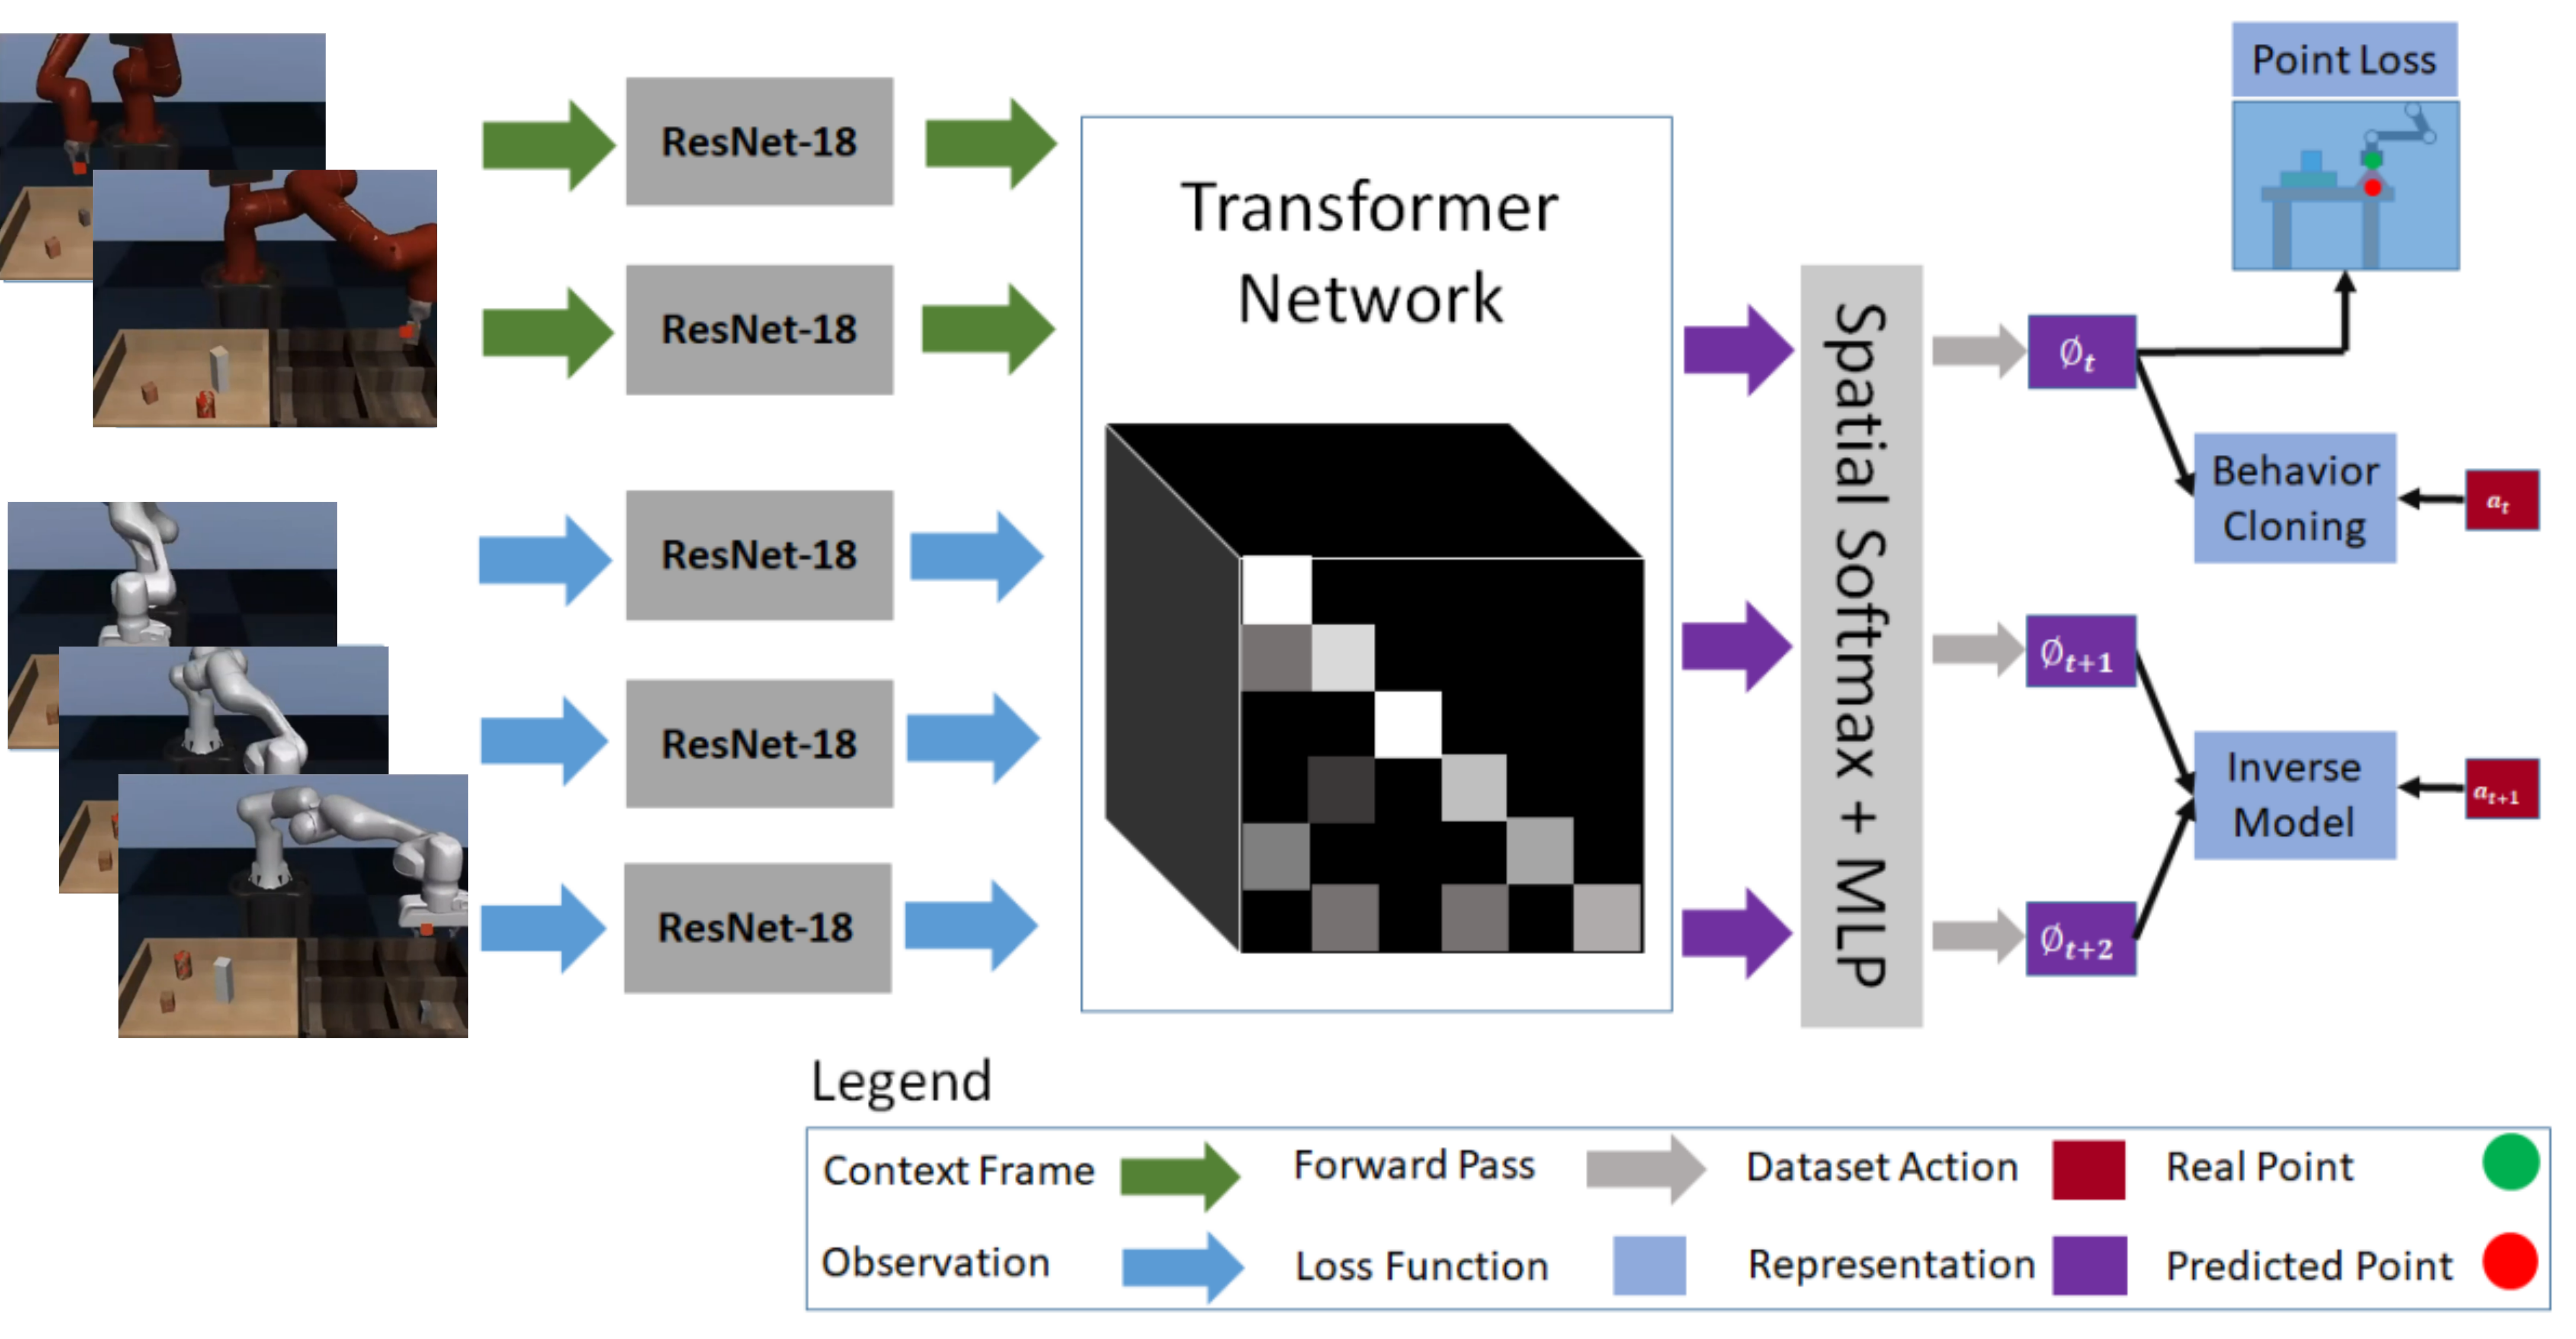
\includegraphics[width=0.7\textwidth]{figures/images/tosil/tosil_architecture.png}
    \caption{Transformer based architecture proposed in \cite{dasari2021transformers_one_shot}.  The Transformer network is used to create task-specific representation, given context and observation features computed with ResNet-18.}
    \label{fig:tosil_architecture}
\end{figure}

\begin{figure}[t]
    \centering
    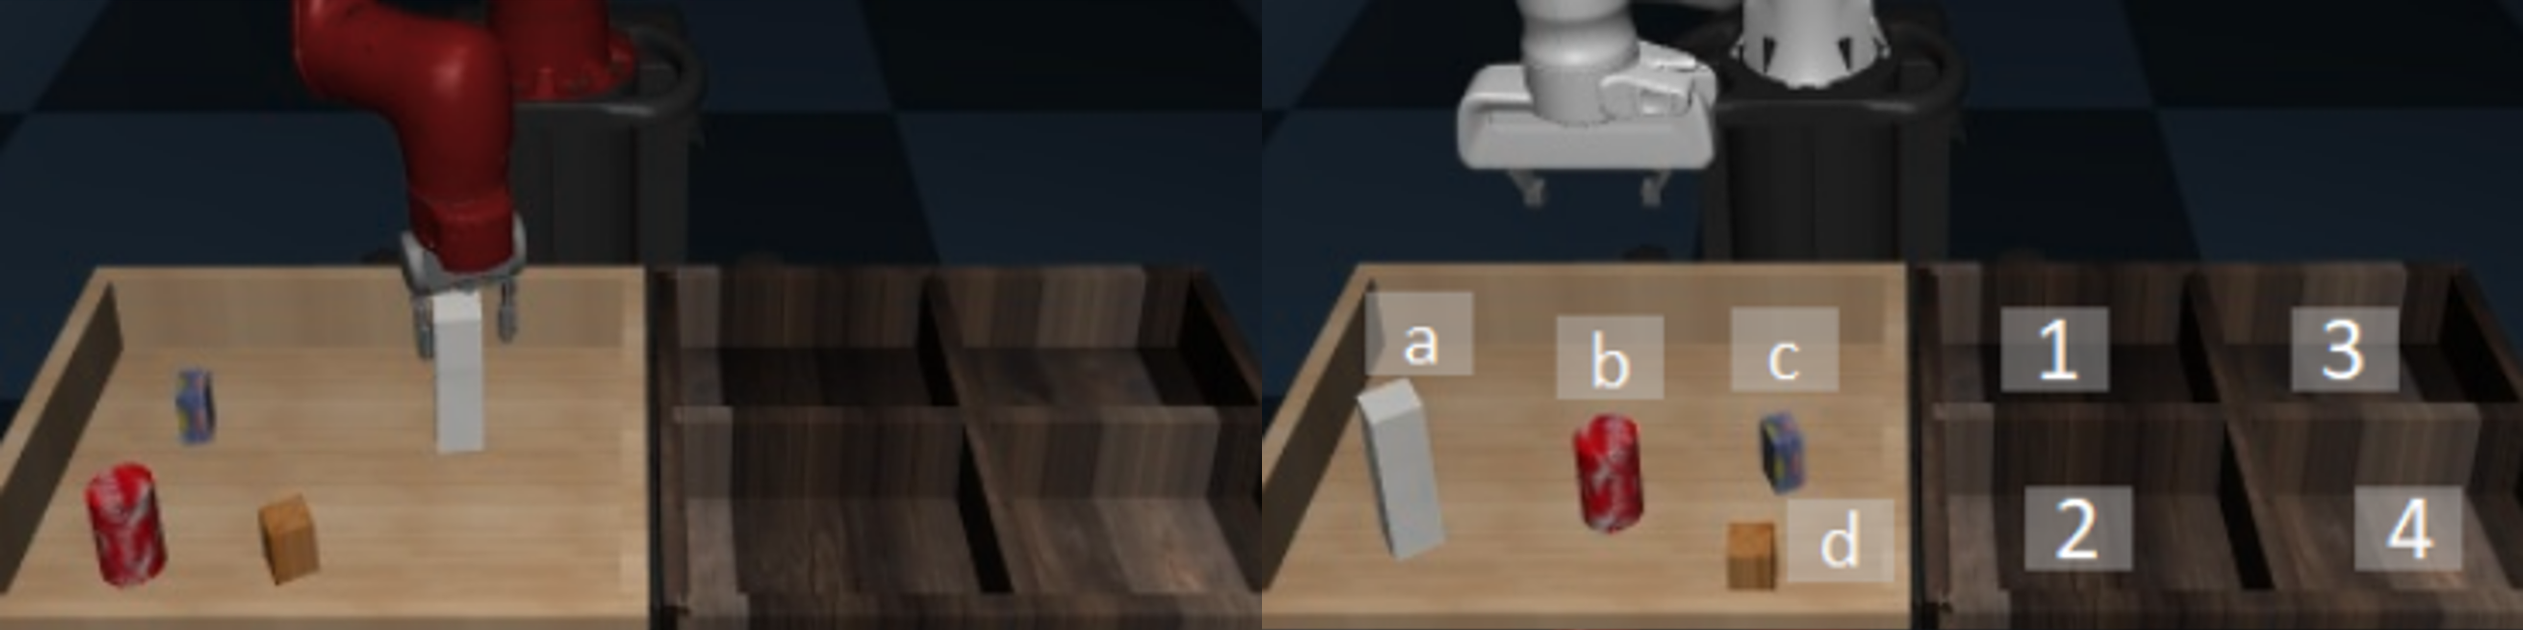
\includegraphics[width=0.7\textwidth]{figures/images/tosil/tosil_task.png}
    \caption{Validation setting proposed in \cite{dasari2021transformers_one_shot}. The
    16 tasks consist of taking an object (a-b) to a bin (1-4). On the left there is the demonstrator robot, while on the right there is the agent robot.}
    \label{fig:tosil_task}
\end{figure}

In \cite{mandi2022towards_more_generalizable_one_shot}, the authors presented MOSAIC (Multi-task One Shot imitation with self-AttentIon and Contrastive learning), which is an improvement of the work proposed in \cite{dasari2021transformers_one_shot} from both the architectural point-of-view and from the evaluation setting.
Indeed, from the architectural point of view, MOSAIC is designed to model a demonstration-conditioned policy, denoted as $\pi^{L}_{\theta}(a_{t}|s_{t},c)$, with $c$ representing the current task demonstration, such as a video depicting a robot performing the task. Specifically, the architecture is an optimization of TOSIL since, where the encoder-decoder Transformer architecture has been substituted with an encoder-only architecture leveraging the self-attention mechanism to correlate the embeddings coming from the current agent observation and the one coming from the demonstration frames (Figure \ref{fig:mosaic_architecture}). This adjustment allows to have a lower number of parameters and consequently improve the inference time. 
\begin{figure}[t]
    \centering
    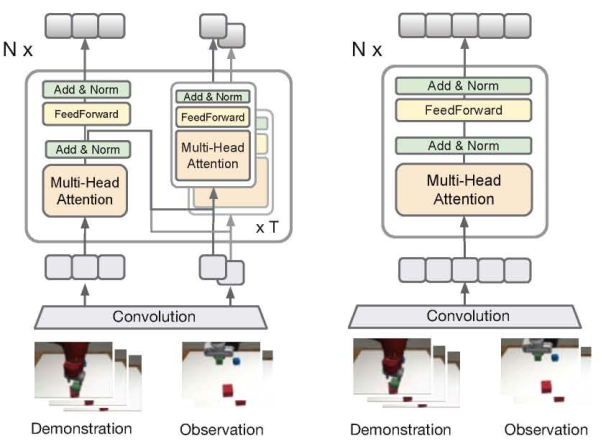
\includegraphics[width=0.7\textwidth]{figures/images/mosaic/architecture_comparison.png}
    \caption{(Left) The TOSIL architecture, as proposed in \cite{dasari2021transformers_one_shot}. (Right) The MOSAIC architecture, as introduced in \cite{mandi2022towards_more_generalizable_one_shot}. In the MOSAIC architecture, the original encoder-decoder Transformer architecture has been replaced with an encoder-only architecture featuring self-attention modules.}
    \label{fig:mosaic_architecture}
\end{figure}

\begin{figure}[t]
    \centering
    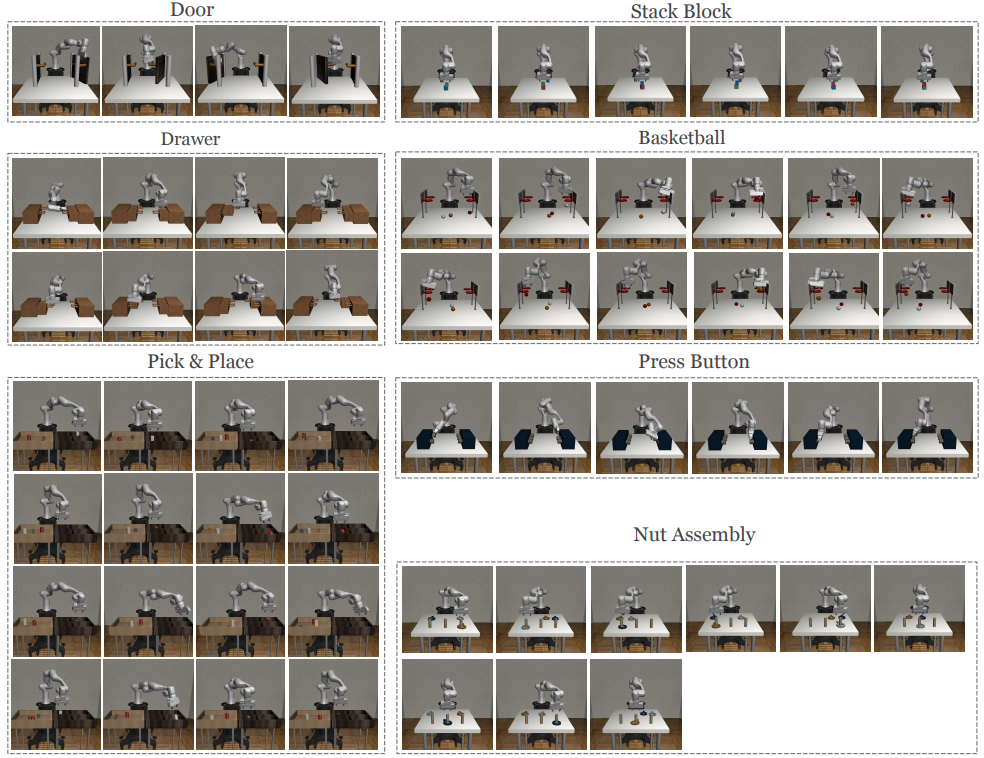
\includegraphics[width=0.7\textwidth]{figures/images/mosaic/mosaic_tasks.png}
    \caption{The evaluation tasks proposed in \cite{mandi2022towards_more_generalizable_one_shot} consist of a total of 7 tasks with 61 semantic variations.}
    \label{fig:mosaic_task}
\end{figure}

To handle this complex scenario involving both multiple variations and multiple tasks, the authors proposed training the system using a combination of loss functions. Specifically, in addition to the $\mathcal{L}_{BC}$ loss function defined in Formula \ref{eq:tosil_bc} and the $\mathcal{L}_{inv}$ loss function defined in Formula \ref{eq:tosil_inv}, the authors introduced a contrastive loss term implemented through the InfoNCE objective (Formula \ref{eq:mosaic_contrastive}). The goal of this loss is to enable the system to create similar representations for time-adjacent frames within a given task while maximizing the distance from representations corresponding to other tasks. In this context, $q$ is the anchor embedding obtained from a randomly sampled frame in a given batch $B$, $k_{+}$ is the positive example, which is a nearby frame from a different view of the batch (i.e., the original batch with a different data augmentation applied), and $k_{i}$ represents the negative samples, obtained from any other frame in the batch.

\begin{equation}
    \label{eq:mosaic_contrastive}
    \mathcal{L}_{Rep} = \log\left(\frac{\exp(q^TWk_{+})}{\exp(q^TWk_{+})+ \sum_{i=1}^{F-1}\exp(q^TWk_{i})}\right)
\end{equation}


To test the model, a dataset containing \textbf{seven distinct tasks} and \textbf{61 variations} (Figure \ref{fig:mosaic_task}) was generated by executing hand-written policies in a simulation environment. This dataset was employed to train and compare the proposed MOSAIC architecture against other one-shot (meta-)imitation learning methods, such as \cite{yu2018daml} and \cite{dasari2021transformers_one_shot}. The results, presented in Table \ref{table:mosaic}, demonstrate that MOSAIC surpasses previous methods in the Single-Task Zero-Shot Imitation Learning setting, particularly when addressing individual tasks with multiple variations and testing on previously unseen scenarios (i.e., novel object configurations).

Furthermore, when evaluated in a Multi-Task setting, where the system is trained on all tasks and subsequently tested on each task separately, MOSAIC exhibits the capability to partially replicate the demonstrated tasks. It is important to note that transitioning from a single-task to a multi-task context introduces inherent challenges. Despite being familiar with the tasks used during training, the success rate tends to decrease for almost all tasks. This phenomenon underscores the necessity for training procedures and architectures capable of generating embeddings that accurately represent both the task itself and its various sub-tasks. Such capacity is essential for reusing these embeddings when executing new instances or entirely novel tasks.

% \usepackage{graphicx}
% \usepackage{multirow}
% \usepackage{hhline}


\begin{table}[t]
    \scriptsize
    \selectfont
    \centering
    \caption{Results obtained in single-task and multi-task one-shot imitation learning \cite{mandi2022towards_more_generalizable_one_shot}.}
    \label{table:mosaic}
    \resizebox{\linewidth}{!}{%
    \begin{tabular}{|c|c|c|c|c|} 
    \hline
    Task & Setup & DAML \cite{yu2018daml} & TOSIL \cite{dasari2021transformers_one_shot} & MOSAIC \cite{mandi2022towards_more_generalizable_one_shot} \\ 
    \hhline{|=====|}
    \multirow{2}{*}{Open door} & single & 23.3~$\pm$ 5.2 & 57.9~$\pm$~7.1 & \textbf{67.1} $\pm$ \textbf{5.5} \\ 
    \cline{2-5}
     & multi & 10.8~$\pm$ 5.4 & 49.2~$\pm$ 6.0 & \textbf{68.3}~$\pm$~\textbf{6.3} \\ 
    \hhline{|=====|}
    \multirow{2}{*}{Open drawer} & single & 15.4~$\pm$ 5.5 & 57.5~$\pm$~3.9 & \textbf{65.4}~$\pm$~\textbf{3.4} \\ 
    \cline{2-5}
     & multi & 3.3~$\pm$~1.4 & 53.3~$\pm$~4.0 & \textbf{55.8}~$\pm$~\textbf{3.6} \\ 
    \hhline{|=====|}
    \multirow{2}{*}{Press button} & single & 62.8~$\pm$~3.9 & 56.4~$\pm$ 2.4 & \textbf{71.7}~$\pm$ \textbf{3.9} \\ 
    \cline{2-5}
     & multi & 1.7~$\pm$~0.7 & 63.3 $\pm$ 3.5 & \textbf{69.4}~$\pm$~\textbf{3.4} \\ 
    \hhline{|=====|}
    \multirow{2}{*}{Pick-and-Place} & single & 0.0~$\pm$~0.0 & 74.4~$\pm$~2.1 & \textbf{88.5}~$\pm$~\textbf{1.1} \\ 
    \cline{2-5}
     & multi & 0.0~$\pm$~0.0 & 19.5~$\pm$~0.4 & \textbf{42.1}~$\pm$ \textbf{2.3} \\ 
    \hhline{|=====|}
    \multirow{2}{*}{Stack block} & single & 10.0~$\pm$~1.8 & 13.3~$\pm$~2.6 & \textbf{79.3}~$\pm$~\textbf{1.8} \\ 
    \cline{2-5}
     & multi & 0.0~$\pm$~0.0 & 34.4~$\pm$~3.4 & \textbf{70.6}~$\pm$~\textbf{2.4} \\ 
    \hhline{|=====|}
    \multirow{2}{*}{Basketball} & single & 0.4~$\pm$~0.3 & 12.5~$\pm$~1.6 & \textbf{67.5}~$\pm$~\textbf{2.7} \\ 
    \cline{2-5}
     & multi & 0.0~$\pm$~0.0 & 6.9~$\pm$~1.3 & \textbf{49.7}~$\pm$~\textbf{2.2} \\ 
    \hhline{|=====|}
    \multirow{2}{*}{Nut assembly} & single & 2.2$\pm$~1.4 & 6.3 $\pm$~1.9 & \textbf{55.2}~$\pm$~\textbf{2.8} \\ 
    \cline{2-5}
     & multi & 0.0~$\pm$~0.0 & 6.3 $\pm$~1.3 & \textbf{30.7}~$\pm$~\textbf{2.5} \\
    \hline
    \end{tabular}
    }
    \end{table}

In this context, further improvements were introduced by the authors of \cite{chang2023one,cui2023from}. Specifically, the authors in \cite{chang2023one} analyze the shortcomings of existing methods like TOSIL and MOSAIC, which often struggle due to issues such as the DAgger problem (distribution shift from offline training), last-centimeter errors in fine motor control (e.g., collisions when the robot reaches the target object to pick), and misalignment with task contexts rather than the actual tasks (e.g., the system links the trajectories to the objects present in the scene rather than focusing on what is demonstrated by the expert).

To overcome these issues, the authors proposed a modular approach that separates task inference, i.e., understanding the intent of the demonstrations, from task execution, i.e., generating the actions to perform during the rollout. To achieve this, they introduced AWDA (Attributed Waypoints and Demonstration Augmentation), a modular framework for visual demonstration represented in Figure \ref{fig:awda_framework}. AWDA is based on two main concepts:

\begin{itemize}
    \item \textit{Attributed Waypoints}, designed to mitigate task execution errors, primarily those related to the distributional shift problem. These are classic waypoints (i.e., sequences of 6D poses of the end-effector) augmented with attributes, such as whether there is an object in the gripper. The robot moves between these generated waypoints using hand-defined motion primitives, which helps eliminate small errors during rollout execution that could otherwise cause the system to deviate from the correct trajectory.
    
    \item \textit{Demonstration Augmentation}, introduced to decouple tasks from task contexts. Specifically, two types of augmentation are introduced: \textbf{Asymmetric Demonstration Mixup}, which generates novel samples by mixing samples from two distinct trajectories according to Formula \ref{eq:awd_blanding}, where $v$ and $\tilde{v}$ are video demonstrations of two distinct tasks, and $o$ and $\tilde{o}$ are agent observations in two distinct contexts. \textbf{Additional Demonstrations via Trajectory Synthesis} involves generating free-space motions for the robot in various contexts by sampling a small number of points (1 to 3) uniformly at random within the agent's workspace and moving the end effector sequentially through these points using an inverse kinematics solver. Training samples are created by pairing each trajectory with itself, requiring the model to focus on the motion of the arm and ignore background elements to make correct predictions.
    
    \begin{equation}
        \label{eq:awd_blanding}
        v'_t = \alpha v_t + (1-\alpha) \tilde{v}_0 \quad o'_t = \alpha o_t + (1-\alpha) \tilde{o}_0
    \end{equation}
    
\end{itemize}
\begin{figure}[t]
    \centering
    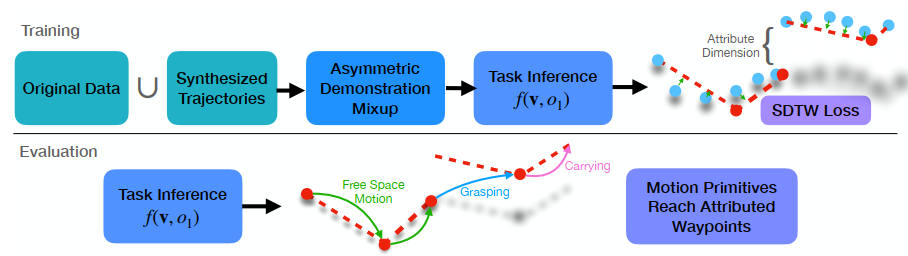
\includegraphics[width=0.9\textwidth]{figures/images/awda/awda_framework.png}
    \caption{AWDA framework proposed in \cite{chang2023one}. The task inference network $f(v,o)$ predicts a sequence of attributed waypoints (red dots) that are achieved by hand-defined motion primitives. The original data are augmented with free-space motion trajectories and asymmetric demonstration mixup in order to reduce the correlation between tasks and task content.}
    \label{fig:awda_framework}
\end{figure}


Using this framework, the authors trained the same Transformer-based architecture as in \cite{dasari2021transformers_one_shot}, achieving notable results. Specifically, on the pick-place task represented in Figure \ref{fig:tosil_task}, AWDA reached a success rate of \textbf{100}\% on two held-out variations, i.e., the system was trained on 14 variations and tested on the remaining 2. However, when tested on completely novel tasks, i.e., tasks never seen during training, the system struggled to succeed, as reported in Table \ref{table:awda_results}.
\begin{table}
    \centering
    \caption{Success rates achieved using the MOSAIC and AWDA methods. In this scenario, training is conducted on 5 out of the 6 tasks, with the remaining task reserved for testing.}
    \label{table:awda_results}
    \resizebox{\linewidth}{!}{%
    \begin{tabular}{|c|c|c|c|c|c|c|} 
    \hline
    Methods & Door & Drawer & Button & Blocks & Basketball & Nut Assembly \\ 
    \hhline{|=======|}
    MOSAIC & \textbf{0.05} & \textbf{0.15} & \textbf{0.05} & 0 & 0 & 0 \\ 
    \hline
    AWDA & \textbf{0.10} & \textbf{0.29} & 0.01 & 0 & 0 & \textbf{0.02} \\
    \hline
    \end{tabular}
    }
    \end{table}

In conclusion, significant research efforts have been dedicated to addressing the challenge of Visual Conditioned Multi-Task Imitation Learning (VC-MTIL). The aim is to develop systems capable of solving a given task in a zero-shot manner, starting from just a single video demonstration. Specifically, while these systems show promising results in solving new instances of seen tasks and unseen variations of known tasks, they struggle to handle a  multi-task multi-variation setting, exhibiting a consistent drop in performance. Additionally, they face difficulties in solving entirely new tasks.

Furthermore, the work discussed in this section predominantly involves experiments conducted in simulation environments, leaving unanswered whether these systems can be effectively applied in real-world settings, where demonstrations might also come in the form of human video demonstrations.
